\chapter{Pr\'esentation du sujet}

\section{Le projet \Yuukou}

\begin{figure}[!ht]
	\centering
	
\includegraphics[scale=1]{yuukouLogo.jpg}

\end{figure}

\subsection{Pr\'esentation}

Le terme Yuukou comme abord\'e dans l'introduction de ce rapport, vient du japonais \Yuukou{} et signifie validit\'e, disponibilit\'e, efficacit\'e.
C'est un syst\`eme permettant la r\'ecup\'eration des informations depuis les serveurs LDAP\protect\footnote{\textit{Lightweight Directory Access Protocol}}$^*$ de l'Universit\'e afin de comprendre et construire l'infrastructure des ressources et ainsi de voir sa facilit\'e d'utilisation. 
L'architecture du syst\`eme utilise un processus d'apprentissage simple pour d\'eduire et maintenir la structure \`a jour avec un minimum de r\'eglages initiaux.
\Yuukou{} a \'et\'e cr\'e\'e pour montrer l'utilisation des salles informatiques et conserver un historique des informations sur le campus de New Cavendish.

\subsection{Fonctionnement}

Le but principal de \Yuukou{} est d'afficher l'occupation des salles informatiques et ce, le plus proche possible d'un syst\`eme fonctionnant en temps r\'eel.
Pour ce faire, l'application a \'et\'e divis\'ee en deux parties  comme le montre la figure~\ref{figure:yuukouFonctionnement}.

\clearpage

\begin{figure}[!ht]
	\centering
	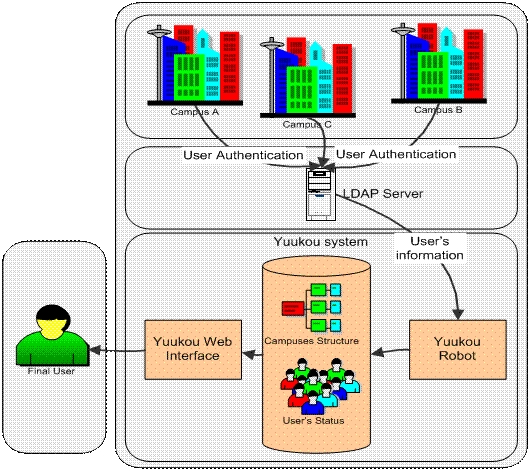
\includegraphics[scale=0.75]{yuukouFonctionnement.jpg}
	\caption{Architecture de \Yuukou}
	\label{figure:yuukouFonctionnement}

\end{figure}

\subsubsection{Premi\`ere partie}

La premi\`ere partie est un programme \'ecrit en Perl$^*$ qui r\'ecup\`ere les informations de connexion des utilisateurs depuis un serveur LDAP$^*$ et qui se charge de construire, modifier ou mettre \`a jour l'architecture r\'eseau de l'Universit\'e tout en stockant les informations dans une base de donn\'ees relationnelle de type MySQL.

Le robot de \Yuukou{} offre deux fonctionnalit\'es : il permet de mettre \`a jour les donn\'ees de connexion via le serveur LDAP$^*$ toutes les cinq minutes environ pour une utilisation normale, et de mettre \`a jour le statut des ressources (ordinateurs) toutes les demi-heures, l\`a aussi pour une utilisation normale.

\subsubsection{Deuxi\`eme partie}

La seconde partie est un ensemble de pages Web \'ecrites en PHP\protect\footnote{\textit{Personal Home Page} ou \textit{PHP: Hypertext Preprocessor}}$^*$ et h\'eberg\'ees sur un serveur Web permettant de pr\'esenter les donn\'ees collect\'ees \`a l'utilisateur final.
Ces pages sont de deux types : les pages publiques et les pages priv\'ees.

Les pages publiques sont accessibles par tous les utilisateurs de l'Universit\'e le d\'esirant.
Les pages priv\'ees, quant \`a elles, ne sont accessibles qu'aux administrateurs.

\subsubsection{Les pages publiques}

\noindent Les pages publiques permettent l'affichage des pages suivantes :

\begin{itemize}
	\item une page contenant tous les campus et salles informatiques actuellement utilis\'ees;
	\item une page par campus avec les salles informatiques actuellement utilis\'ees;
	\item une page par campus et d\'epartement avec les salles informatiques actuellement utilis\'ees.

\end{itemize}

\vspace{0.20cm}

Les pages publiques offrent une vision g\'en\'erale de chaque salle : le nombre de ressources totales, disponibles, occup\'ees par un utilisateur et dans un \'etat inconnu.
Il est \`a noter que chacunes des pr\'ec\'edentes pages peut \^etre affich\'ees sur un \'ecran plasma pr\'esent dans les diff\'erents b\^atiments de l'Universit\'e.
La figure~\ref{figure:yuukouPublic} donne un exemple de page publique.

\subsubsection{Les pages priv\'ees}

\noindent Les pages priv\'ees permettent l'affichage des pages suivantes :

\begin{itemize}
	\item une page d'identification via LDAP$^*$ pour l'administrateur;
	\item toutes les pages publiques mais b\'en\'eficiant de fonctionnalit\'es suppl\'ementaires :

	\begin{itemize}
		\item liste des ressources \'eteintes;
		\item une fen\^etre permettant d'avoir des informations sur un utilisateur actuellement connect\'e \`a une ressource (identifiant, nom, photo, heure de connexion et dur\'ee de la session);
		\item possibilit\'e d'ajouter des commentaires sur les utilisateurs;
		\item liens vers les statistiques des salles informatiques.

	\end{itemize}

\end{itemize}

\vspace{0.20cm}

La figure~\ref{figure:yuukouAdmin} donne un exemple des fonctionnalit\'es suppl\'ementaires auxquelles un administrateur a acc\`es.

\clearpage

\subsubsection{Vue sur le produit}

\begin{figure}[!ht]
	\centering
	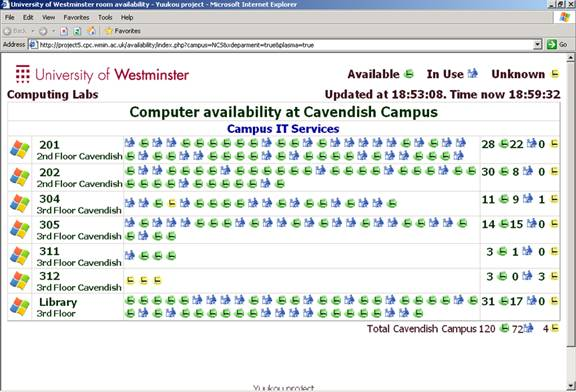
\includegraphics[scale=0.75]{yuukouPublic.jpg}
	\caption{Exemple de page publique de \Yuukou{} rep\'esentant un campus et l'utilisation des salles informatiques d'un d\'epartement}
	\label{figure:yuukouPublic}

\end{figure}

\begin{figure}[!ht]
	\centering
	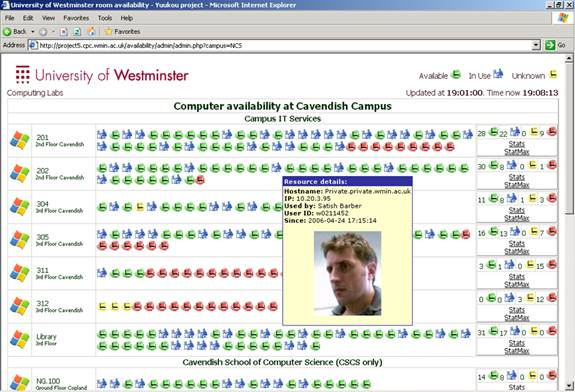
\includegraphics[scale=0.75]{yuukouAdmin.jpg}
	\caption{Exemple de page priv\'ee de \Yuukou{} montrant en particulier les donn\'ees d'un utilisateur}
	\label{figure:yuukouAdmin}

\end{figure}

\subsection{Quelques Chiffres}

Le projet \Yuukou{} permet de surveiller le r\'eseau du campus de New Cavendish soit 43 salles informatiques, ce qui repr\'esente 661 PC. 
Le support des Macintosh n'\'etant pas pris en compte.

\subsection{Changement vers \YuukouII}

L'Universit\'e souhaite reprendre le principe du projet \Yuukou, cependant elle est confront\'ee \`a diff\'erents probl\`emes.
Le premier \'etant que les personnes ayant d\'evelopp\'e le projet ont quitt\'e l'Universit\'e. 
Ce qui signifierait, pour la personne ou l'\'equipe en charge d'\'eventuellement reprendre le projet, de prendre du temps pour se former \`a Perl$^*$, comprendre tout ce qui a \'et\'e d\'ej\`a r\'ealis\'e et ensuite seulement, commencer \`a d\'evelopper.
Actuellement de nombreux projets sont en cours et il n'est pas possible pour une \'equipe de passer du temps sur l'existant.

Un autre probl\`eme est les changements importants, du point de vue infrastructure, qui sont en train d'\^etre mis en place.
En effet, l'Universit\'e qui utilisait eDirectory$^*$ de Novell pour g\'erer ses annuaires LDAP$^*$ a commenc\'e \`a migrer toutes ses donn\'ees vers le syst\`eme Active Directory$^*$ de Microsoft qui est cens\'e \^etre plus efficace. Ce changement rendrait \Yuukou{} obsol\`ete.

Point suivant, la volont\'e de donner acc\`es aux informations sur les salles, pas seulement en utilisant un navigateur Internet, mais aussi et surtout en utilisant un \textit{smartphone} (IPhone ou autres par exemple) ou une tablette (IPad par exemple), chose que l'ancien logiciel ne peut pas fournir.
De ce fait, un \'etudiant aurait \`a tout moment les informations sur les salles via son \textit{smartphone} ou sa tablette, si tant est qu'il ait l'un ou l'autre.

\noindent \`A ces pr\'ec\'edents probl\`emes, d'autres viennent s'ajouter :

\begin{itemize}
	\item les Macintosh ne sont pas pris en compte;
	\item le logiciel est assez monolithique donc il deviendrait tr\`es difficile et complexe de vouloir l'\'etendre;
	\item {\Yuukou} ne prend en compte que les donn\'ees en temps r\'eel et ne garde pas un historique;
	\item son utilisation pr\^ete \`a confusion car il n'a aucun interfa\c{c}age avec l'emploi du temps, de ce fait, quand une salle est pr\'esent\'ee comme libre, il n'y a aucun moyen, avec le logiciel, de savoir si un cours s'y d\'eroule ou non.

\end{itemize}

\vspace{0.20cm}

C'est en consid\'erant tous ces points qu'il a \'et\'e d\'ecid\'e d'abandonner le projet \Yuukou{} afin de pouvoir mettre en place \YuukouII{} qui r\'epondrait aux attentes de l'Universit\'e.

\section{Le projet \YuukouII}


\YuukouII{} a pour but de combler les lacunes de \Yuukou{} et d'aller plus loin en termes de fonctionnalit\'es qu'il peut offrir. 
Dans son fonctionnement g\'en\'eral, il doit permettre de donner \`a un \'etudiant ou toute personne travaillant \`a l'Universit\'e et cherchant \`a utiliser un ordinateur, une vue globale des ressources qui sont disponibles actuellement.
Les donn\'ees devant \^etre bien s\^ur exactes afin que la personne n'ait pas de mauvaise surprise en se rendant dans une salle qu'elle pensait libre.
L'affichage pourra se faire via un \textit{smartphone}, une tablette ou encore un navigateur Internet.

\noindent Le but du stage est : 

\begin{itemize}
	\item la conception d'un logiciel permettant la r\'ecup\'eration de donn\'ees concernant les connexions sur les diff\'erentes ressources de l'Universit\'e et cela en temps r\'eel;
	\item la gestion de la persistance de ces donn\'ees;
	\item la cr\'eation d'un maximum de fonctionnalit\'es retournant les informations utiles dans le but d'\^etre exploit\'ees pour l'affichage sur les diff\'erents supports.

\end{itemize} 

\vspace{0.20cm}

La cr\'eation d'applications permettant l'affichage des r\'esultats ne fait pas partie de ce sujet de stage. 
Ici, seule la partie r\'ecup\'eration, stockage et retour des donn\'ees est abord\'ee.

\clearpage
